\chapter{Spectral Method}
\label{chap:spectral-method}

\begin{theorem}{Integration Theorem that needs a name}{theorem216}
  On the $d$-dimensional unit ball $B_1$ the power law potential, with power $\alpha \in(-d,2+2m-d)$, $m\in\mathbb{N}_0$ and $\beta>-d$, of the $n$-th weighted radial Jacobi polynomial $$(1-|y|^2)^{m-\frac{\alpha+d}{2}}P_n^{(m-\frac{\alpha+d}{2},\frac{d-2}{2})}(2|y|^2-1)$$ reduces to a Gaussian hypergeometric function as follows:
  \begin{align*}
    \int_{B_1} & |x-y|^\beta (1-|y|^2)^{m-\frac{\alpha+d}{2}} P_n^{(m-\frac{\alpha+d}{2},\frac{d-2}{2})}(2|y|^2-1) \mathrm{d}y                                                                                                                                                                                                                                                                                               \\
               & = \tfrac{\pi ^{d/2} \Gamma \left(1+\frac{\beta}{2}\right) \Gamma \left(\frac{\beta+d}{2}\right) \Gamma \left(m+n-\frac{\alpha+d}{2}+1\right)}{\Gamma \left(\frac{d}{2}\right) \Gamma (n+1) \Gamma \left(\frac{\beta}{2}-n+1\right) \Gamma \left(\frac{\beta-\alpha}{2}+m+n+1\right)}{}_2F_1\left(\begin{matrix}n-\frac{\beta}{2}, \quad -m-n+\frac{\alpha-\beta}{2} \\\frac{d}{2}\end{matrix};|x|^2\right).
  \end{align*}
\end{theorem}

\section{Derivation of Operator}
Based on the {[}{[}Three-Term Recurrence Relationship{]}{]}.

One can even determine an explicit relationship between the coefficients
in the Jacobi expansion by considering the {[}{[}Jacobi Matrix{]}{]}.

Considering the operator $\hat{Q}^\beta[\rho]$ as in \Cref{thm:theorem216}, from the [[Ansatz]] $\rho(x)$ we have
$$\hat{Q}^{\beta}(x) = \sum_{k=1}^{N} \rho_{k} \int \norm{x-y}^{\beta}(1-\norm{y}^2)^{a}P_{k}^{(a, b)}(2\norm{y}^{2}- 1) \,\ddy$$


\begin{figure}[H]
  \centering
  \label{fig:attractive-repulsive}
  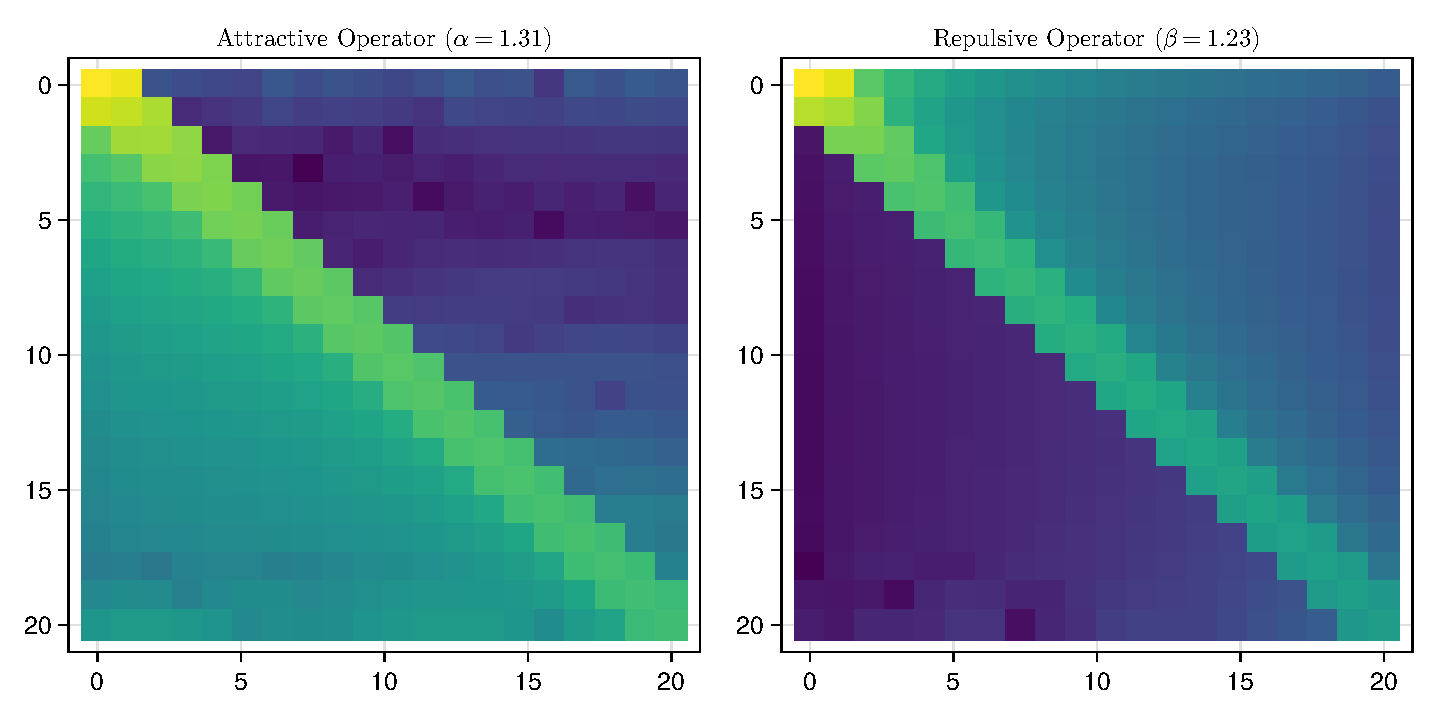
\includegraphics[width=\linewidth]{../figures/results/attractive-repulsive-operator.pdf}
  \caption{The attractive and repulsive operators}
\end{figure}
